% DUET -- Evaluation (DAC 2027 draft, 2026-11-01), rough: figures placed, text to be written.
% Figures: tools/plot_eval.py -> results/paper_dac/fig_eval_{read,write,tput}.pdf, data in results/paper_dac/eval_data.csv.
% Bounded FTLs (DUET, DFTL, LeaFTL, CoMap; uFTL dropped from the figures) = results/final_vbm. Page, FAST, IU+RMW = results/final_rp (traces, apps)
% and results/final_rp_a128 (raw I/O).
% Raw I/O: 4K:128K = 70:30 only, labelled by R:W (2026-11-06). Geomean over the 10 workloads, normalized to Page:
% throughput DUET 0.93, LeaFTL 0.73, DFTL 0.67, IU+RMW 0.66, FAST 0.57, CoMap 0.46.
% Avg. read DUET 1.03, FAST 1.51, IU+RMW 1.61, LeaFTL 1.65, CoMap 1.81, DFTL 2.41.
% Avg. write DUET 0.93, DFTL 0.74, LeaFTL 1.27, FAST 2.40, IU+RMW 2.76, CoMap 3.33.
% p99 read DUET 1.02, FAST 1.35, CoMap 1.67, IU+RMW 1.70, DFTL 1.71, LeaFTL 2.10.
% p99 write DUET 0.75, DFTL 0.71, LeaFTL 0.99, IU+RMW 2.15, FAST 2.50, CoMap 3.65.

\section{Evaluation}
\label{sec:eval}

\textbf{Setup.} TODO: NVMeVirt configuration, OP 7\%, 1/8 mapping DRAM, the seven FTLs, workloads.

\begin{figure*}[t]
  \centering
  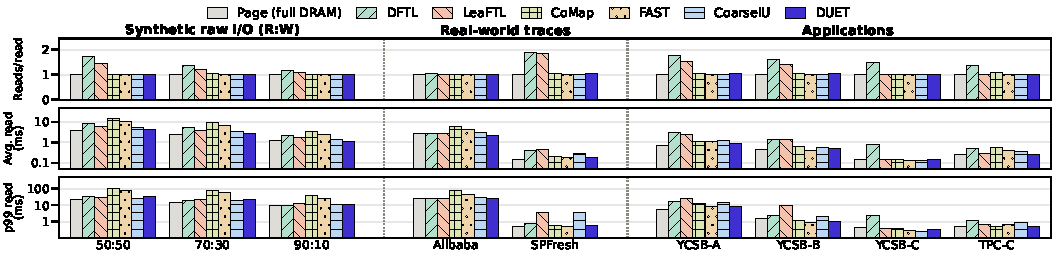
\includegraphics[width=\textwidth]{figs/fig_eval_read.pdf}
  \vspace{-6mm}
  \caption{Read path. From top, flash reads per host read (data plus mapping reads), and average and p99 read latency.}
  \label{fig:eval-read}
  \vspace{-3mm}
\end{figure*}

\begin{figure*}[t]
  \centering
  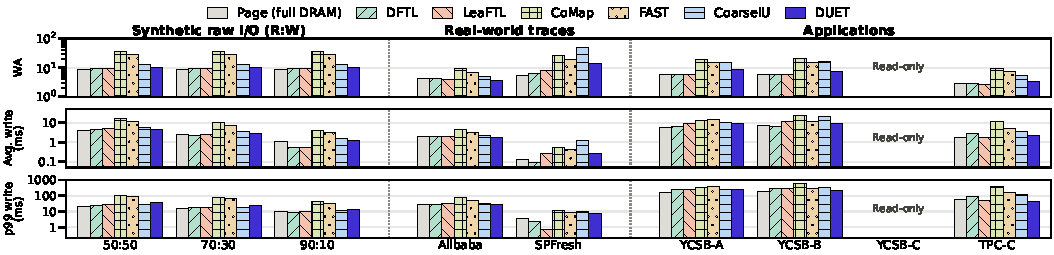
\includegraphics[width=\textwidth]{figs/fig_eval_write.pdf}
  \vspace{-6mm}
  \caption{Write path. From top, device write amplification, and average and p99 write latency.}
  \label{fig:eval-write}
  \vspace{-3mm}
\end{figure*}

\begin{figure*}[t]
  \centering
  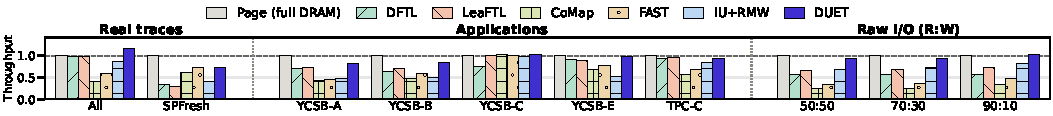
\includegraphics[width=\textwidth]{figs/fig_eval_tput.pdf}
  \vspace{-6mm}
  \caption{Throughput normalized to Page.}
  \label{fig:eval-tput}
  \vspace{-3mm}
\end{figure*}

\textbf{Read latency.} TODO (Figure~\ref{fig:eval-read}).

\textbf{Write amplification and write latency.} TODO (Figure~\ref{fig:eval-write}).

\textbf{Throughput.} TODO (Figure~\ref{fig:eval-tput}).

% Ablation: tools/plot_ablation.py -> results/paper_dac/fig_ablation.{pdf,png}, data in ablation_data.csv.
% Build-up: Basic = nsfm (spill=0, fold_all=1, gc_select_cost=0), + victim selection = nsm, + copy-or-merge = ns,
% + spill/load = DUET (final_vbm). Variants = final_ablation. Normalized to Basic.
\begin{figure}[t]
  \centering
  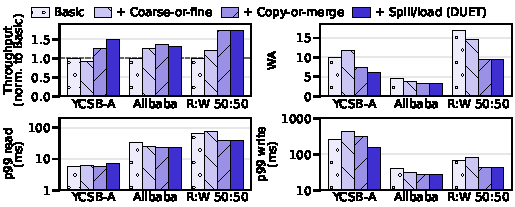
\includegraphics[width=\columnwidth]{figs/fig_ablation.pdf}
  \vspace{-6mm}
  \caption{Ablation. From left to right, each bar adds one more technique to Basic, and the rightmost bar is DUET. Throughput is normalized to Basic.}
  \label{fig:eval-ablation}
  \vspace{-4mm}
\end{figure}

\textbf{Ablation.} TODO (Figure~\ref{fig:eval-ablation}).
